\begin{figure}[!t]
\centering
\includegraphics[width=0.7\textwidth, clip=true]{./Chapters/02_Registration/Images/./EpiRegistration}
%\includegraphics[width=0.8\textwidth, clip=true]{./Chapters/02_Registration/Images/./Images/EpiRegistration.png}
\caption{
	Distortion correction of 7T 3D EPI data, obtained with 0.93 mm isotropic resolution. In {\color{red}red}, the original brain surfaces are shown after a 12 DoF registration performed by \texttt{bbregister}. The mesh in {\color{green}green} is the updated mesh by means of the first stage RBR, 2 DoF (scale and translation in the PE direction). The green boundaries follow the white matter boundary much better. The voxel displacement map (lower right) shows displacements on the order of several millimetres. The control point lattice that was used to displace the boundaries are overlaid onto the displacement map. Similar images for all subjects can be found in the supplementary materials. For even better inspection, movie files for all subjects are included in supplementary figure~\ref{fig:si-registrations}.} 
\label{fig:epiregistration}
\end{figure}